\chapter{Casos de Estudio}
\todomm{intro}
\section{Ejemplo de demostraci'on con file system}
\todomm{Reescribir esta sección siguiendo las guías que vas a ver más adelante. Además, así como está no se ven las funcionalidades nuevas. Incluir alguna búsqueda de contraejemplos, bifurcación en alternivas de demostración y traducción de fórmulas en este mismo ejemplo.}

\todomm{Explicá también de qué se trata la especificación}
Para demostrar \todomm{Hablar de “ejemplo de uso”}el uso de Heterogenius en un caso real recurrimos a la demostraci'on de la propiedad \textit{NoDirAliases} definida en el archivo de especificaci'on Alloy \textit{$file\_system.als$} \ref{anexo_fs}. \todomm{No poner el número de anexo solo. Decir que la especificación puede encontrarse en ese apéndice y que es una adaptación del ejemplo homónimo del libro de jackson (y poner referencia)

@book{Jackson:2006:SAL:1146359,
 author = {Jackson, Daniel},
 title = {Software Abstractions: Logic, Language, and Analysis},
 year = {2006},
 isbn = {0262101149},
 publisher = {The MIT Press},
} 

Esta también es la referencia para cuando hables de Alloy}

Lo primero que se hace al abrir Heterogenius es cargar la especificaci'on con la que se va a trabajar y seleccionar la propiedad que se quiere demostrar:

\todomm{De este tipo de figuras, donde aparecen las tres ventanas de heterogeniuos, sólo poner una. Explicar para qué sirve cada ventana y después sólo mostrar los árboles.}
\begin{figure}[H]
	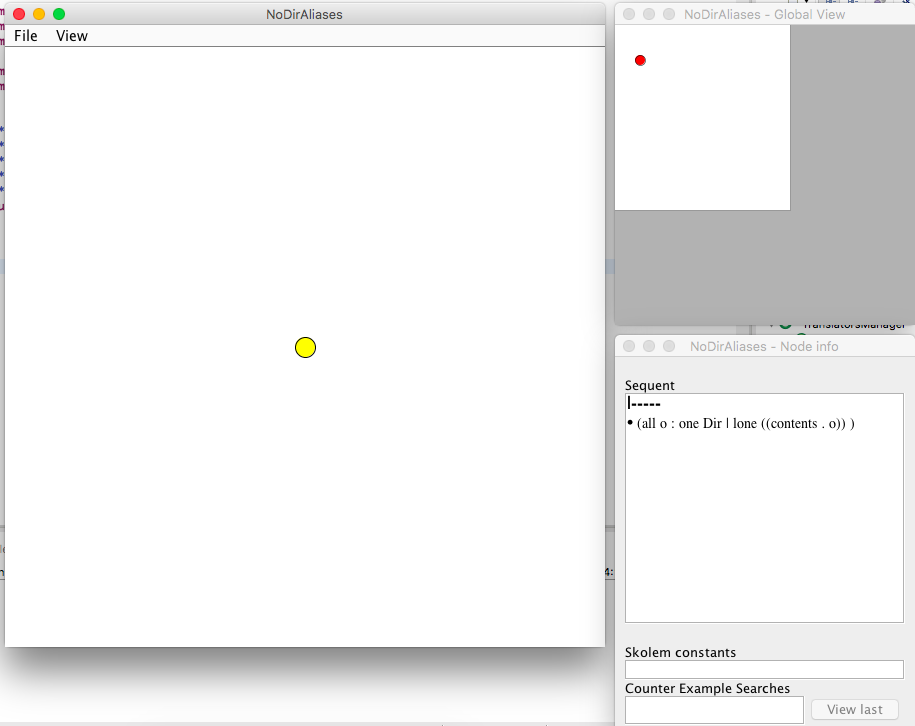
\includegraphics[width=350px]{img/ejemplo/3.png}
	\centering
	\caption{La propiedad cargada aparece como un 'unico nodo del 'arbol de demostraci'on}
\end{figure}

En la ventana \textit{Node Info} se puede ver el detalle del nodo seleccionado. As'i, la propiedad a demostrar es:

\begin{verbatim}
all o: one this/Dir | lone (contents.o)
\end{verbatim}

Lo primero que se puede hacer es aplicar una skolemizaci'on para eliminar el cuantificador universal:

\begin{figure}[H]
	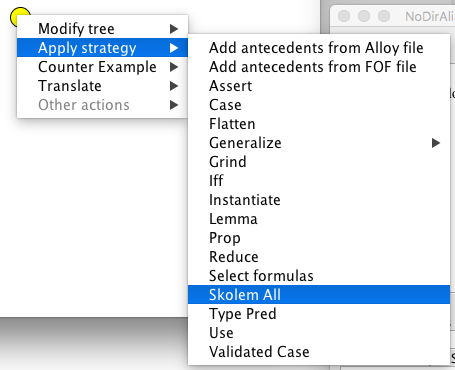
\includegraphics[width=250px]{img/ejemplo/4.png}
	\centering
	\caption{Se selecciona 'Skolem all' desde la lista de estrategias.}
\end{figure}

La aplicaci'on de dicha acci'on crear'a un nodo nuevo en el 'arbol de demostraci'on con la nueva expresi'on a demostrar.

\todomm{No poner cada paso como una firgura aparte. Simplemente intercalar los árboles (pequeños) en el texto }
\begin{figure}[H]
	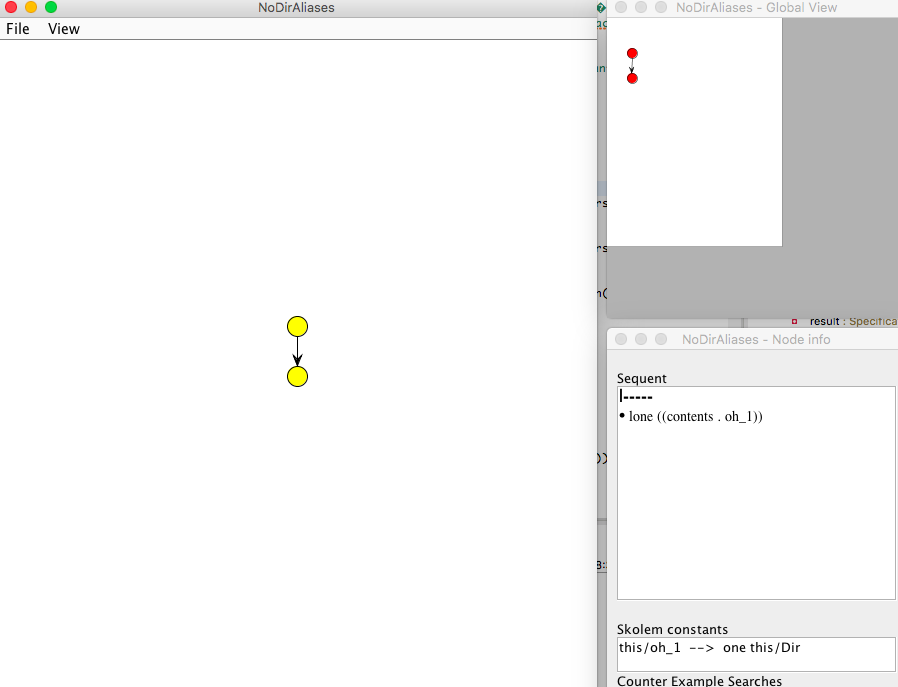
\includegraphics[width=350px]{img/ejemplo/5.png}
	\centering
	\caption{}
\end{figure}

El siguiente paso ser'a separar el nodo en casos seg'un la expresi'on $oh\_1$ $in$ $Root$. Para 'esto se selecciona la opci'on \textbf{Case} desde la lista de estrategias y se ingresa la expresi'on:

\todomm{de las siguientes 2 figuras poner las ventanas con formulas y un arbol}
\begin{figure}[H]
	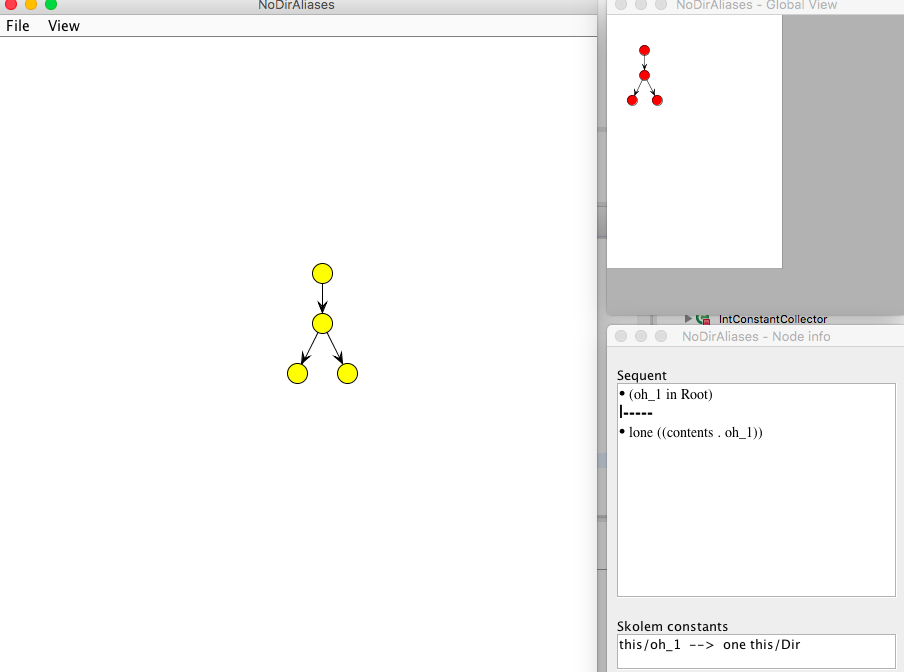
\includegraphics[width=350px]{img/ejemplo/7.png}
	\centering
	\caption{Nodo de la izquierda representa el caso 1}
\end{figure}

\begin{figure}[H]
	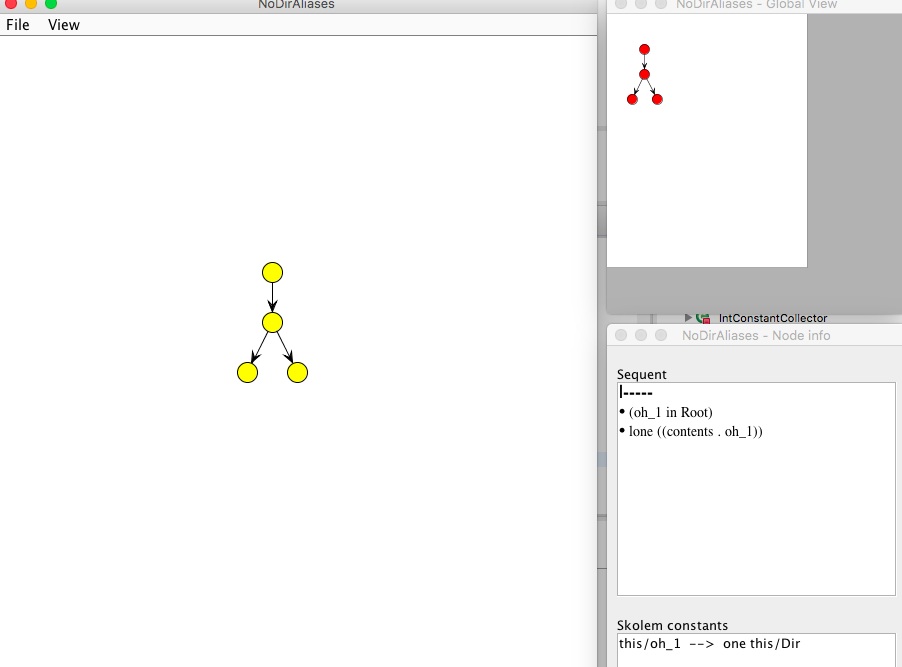
\includegraphics[width=350px]{img/ejemplo/8.png}
	\centering
	\caption{Nodo de la derecha representa el caso 2}
\end{figure}

El nodo sobre el que se aplic'o la acci'on \textbf{Case} se subdivide en dos nodos hijos, cada uno representando un caso posible. Las ramas con lineas solidas indican que es necesario demostrar ambas ramas para concluir con la demostraci'on del nodo padre.

\subsection{Demostraci'on del caso 1}

Empecemos con la primer rama. Lo primero que se puede hacer es introducir uno de los lemas definidos en el archivo de especificaci'on cargado. En particular se puede probar con el lema \textit{RootHasNoParent}:

\begin{figure}[H]
	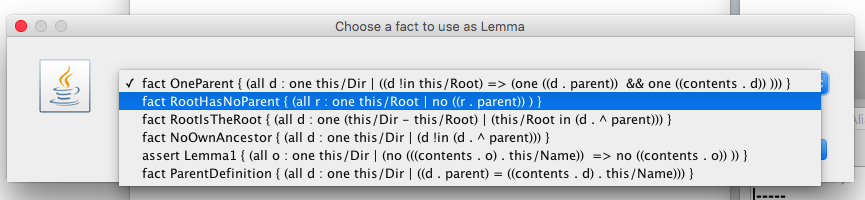
\includegraphics[width=350px]{img/ejemplo/9.png}
	\centering
	\caption{Al seleccionar la opci'on \textbf{Use} de la lista de las estrategias se presenta un dialogo para elegiar el lemma a introducir.}
\end{figure}

\begin{figure}[H]
	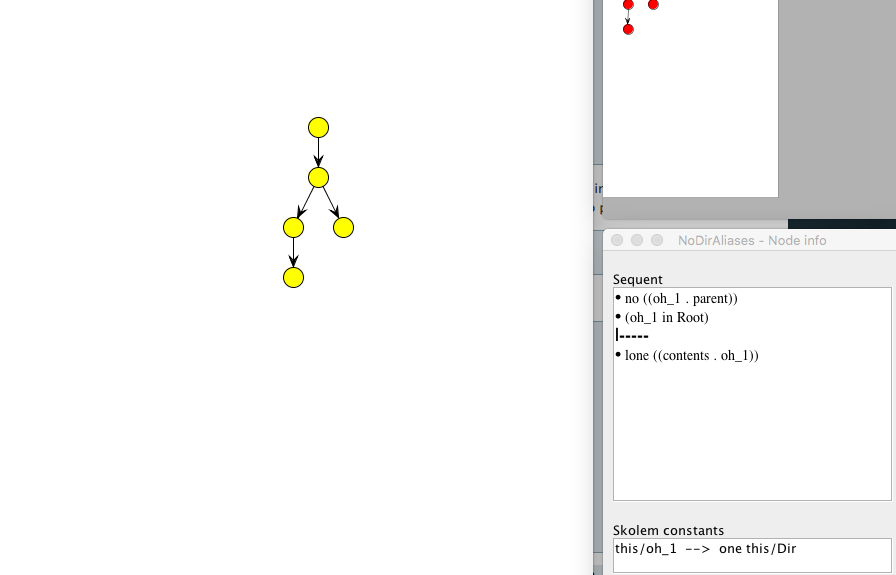
\includegraphics[width=350px]{img/ejemplo/10.png}
	\centering
	\caption{La aplicaci'on del lemma resulta en un nodo nuevo.}
\end{figure}

A continuaci'on se introduce el lemma: \textit{ParentDefinition}:

\begin{figure}[H]
	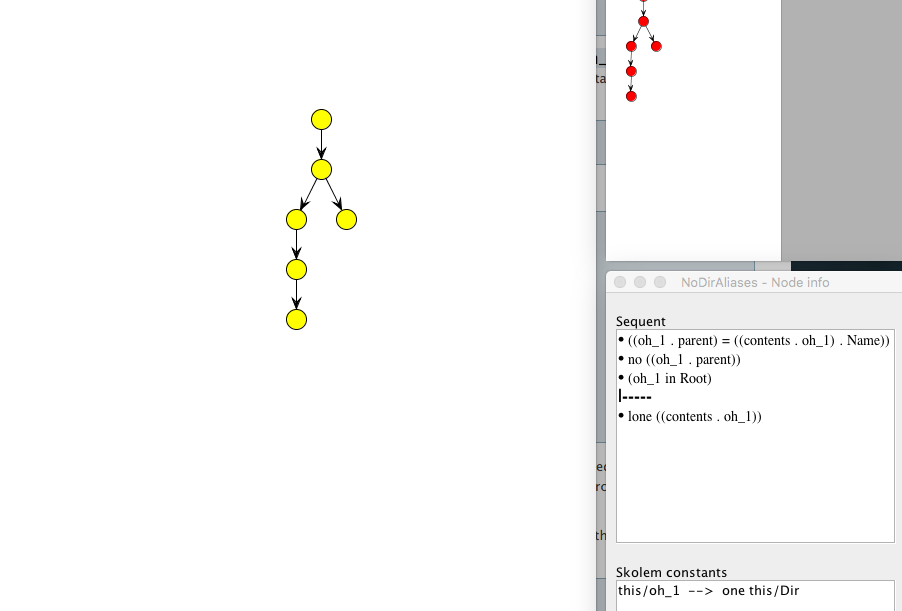
\includegraphics[width=350px]{img/ejemplo/12.png}
	\centering
	\caption{Nodo resultante luego de introducir el lemma \textit{ParentDefinition}}
\end{figure}

Se introduce el lema \textit{Lemma1} definido en el archivo de especificaci'on como:

\begin{verbatim}
all o: Dir | no contents.o . Name => no contents.o
\end{verbatim}

\begin{figure}[H]
	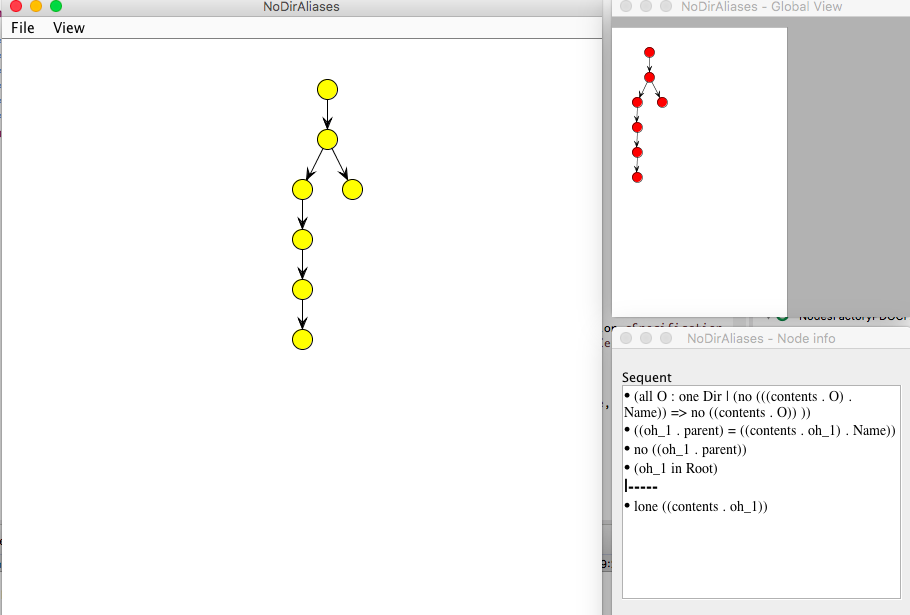
\includegraphics[width=350px]{img/ejemplo/13.png}
	\centering
	\caption{}
\end{figure}

Para terminar con la demostraci'on de 'esta rama se aplica la estrategia \textbf{Reduce}

\begin{figure}[H]
	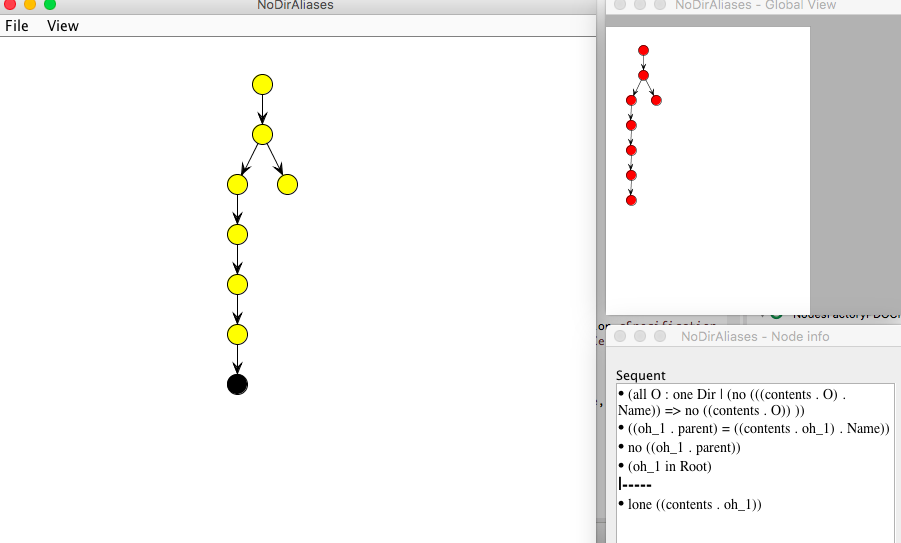
\includegraphics[width=350px]{img/ejemplo/14.png}
	\centering
	\caption{}
\end{figure}

\subsection{Demostraci'on del caso 2}

El nodo a demostrar de la segunda rama es:

\begin{prooftree}
\AxiomC{}
\UnaryInfC{$oh\_1$ $in$ $Root$}
\noLine
\UnaryInfC{$lone$ $(contents$ . $oh\_1)$}
\end{prooftree}


Lo primero que se puede hacer es aplicar la propiedad \textbf{OneParent} definia como:

\begin{verbatim}
all d: one this/Dir | (d !in this/Root) => (one (d . parent)
		&& one (contents . d) )
\end{verbatim}

con lo cu'al esta expresi'on se agrega a las hip'otesis del nodo y aplicando a continuaci'on \textbf{reduce} y \textbf{grind} se llega a completar la demostraci'on de la rama:

\begin{figure}[H]
	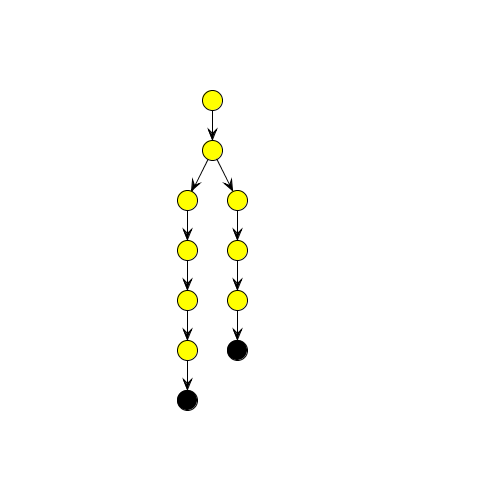
\includegraphics[width=250px]{img/ejemplo/15.png}
	\centering
	\caption{Los nodos negros indican que las ramas est'an demostradas.}
\end{figure}

Ya que todos los pasos aplicados preserva la verdad y como los nodos hojas de ambas ramas quedaron demostrados, el nodo ra'iz del 'arbol de demostraci'on tambi'en queda demostrado.


\section{B'usqueda de contraejemplo}

A continuaci'on se ejemplifica el an'alisis de una conjectura definida en el lenguaje \textit{Alloy}:

\begin{verbatim}
assert ConjeturaFalsa {
    all o: Dir | some (contents.o)
}
\end{verbatim}

La especificaci'on que se usa para este ejemplo es \textit{file$\_$system.als} \ref{anexo_fs}

Lo primero que se hace es cargar el archivo de especificaci'on que contiene dicha conjecura (\textbf{File$\rightarrow$New Analysis$\rightarrow$Alloy}). Una vez hecha la carga, lo que se quiere demostrar aparece en el nodo ra'iz:

A continuaci'on, como se quiere hacer el an'alisis con herramientas de \textit{TPTP-FOF}, es necesario traducir el secuente analizado a \textit{PDOCFA} y luego a \textit{TPTP-FOF}. Las traducciones se realizan seleccionando la opci'on \textbf{$\rho$-translate to PDOCFA} del men'u que aparece al hacer click derecho sobre el nodo ra'iz; y luego aplicando \textbf{$\rho$-translate to TPTP-FOF} haciendo click derecho sobre el nodo resultante de la operaci'on anterior. 

'Esto crea dos nodos nuevos en el 'arbol, representando cada acci'on realizada y mostrando el secuente resultante de las acciones aplicadas:

\begin{figure}[H]
	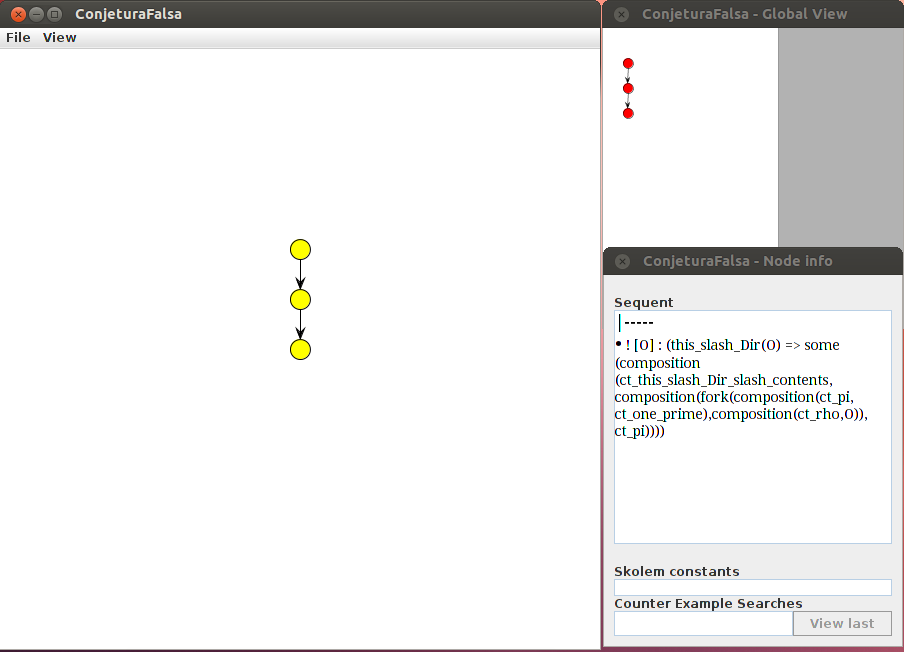
\includegraphics[width=350px]{img/conjetura_falsa_2.png}
	\centering
	\caption{El nodo hoja seleccionado, representa la conjetura inicial traducida al lenguaje \textit{TPTP-FOF}}
\end{figure}

Intuitivamente sospechamos que la conjetura debe ser falsa, ya que est'a diciendo que ``todos los directorios tienen alg'un contenido''. Teniendo 'esto en cuenta, primero probamos realizar una b'usqueda de un contraejemplo con \textit{EProver}, haciendo click derecho sobre el nodo hoja y seleccionando \textbf{Counter Example$\rightarrow$Find Counter Example using EProver for TPTP-FOF}.

Luego de unos segundos el sistema indica que no se pudo encontrar un contraejemplo. Este mensaje no indica que el contraejemplo no existe y solamente nos dice que la herramienta no lo encontr'o. Con lo cu'al se puede seguir buscando con otra herramienta.

C'omo ya se realiz'o una acci'on sobre el nodo hoja y no queremos perder la informaci'on del resultado de 'esta acci'on, lo que se hace es crear una rama alternativa para seguir con la demostraci'on manteniendo los resultados en una rama aparte. Al hacer click derecho sobre el nodo y seleccionando \textbf{Modify Tree$\rightarrow$Create an alternative branch} se abren dos ramas salientes del nodo seleccionado. Cada rama est'a representada por una copia del nodo y puede ser analizada en forma independiente del resto.

\begin{figure}[H]
	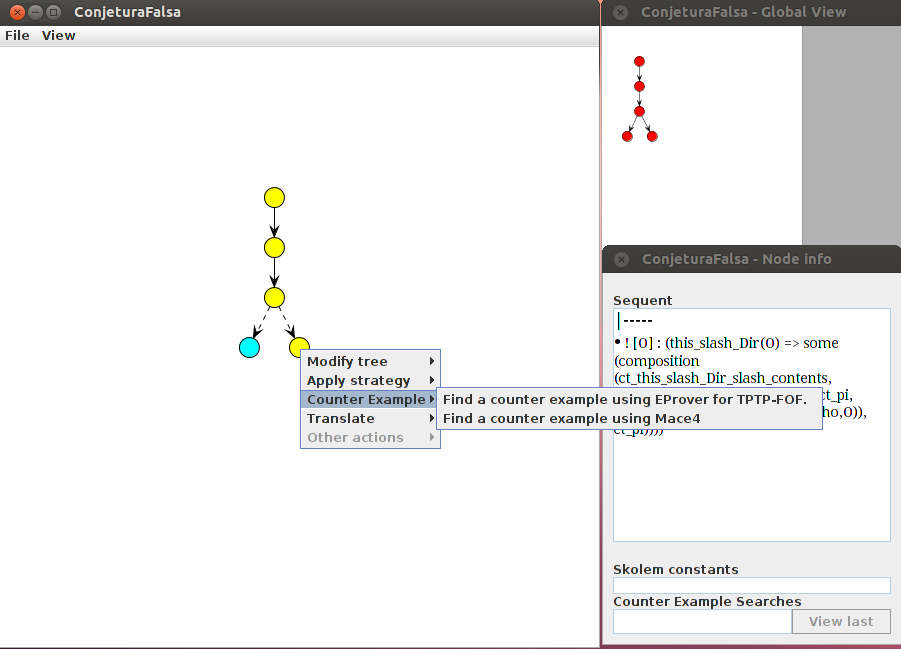
\includegraphics[width=350px]{img/conjetura_falsa_3.png}
	\centering
	\caption{Nodo celeste indica que no se encontr'o un contraejemplo.}
\end{figure}

'Esta ramificaci'on representada con una l'inea punteada se interpreta como un camino alternativo. Alcanza con llegar a un resultado en una de las ramas para afirmar que el resultado vale para el nodo ra'iz de la ramificaci'on.

Para seguir buscando se intenta una b'usqueda de contraejemplo con otra herramienta, \textit{Mace4}. Al hacer click sobre el nodo de la rama derecha y seleccionando \textbf{Counter Example$\rightarrow$Find a counter example using Mace4} se lanza la operaci'on.

'Esta vez se logra encontrar un contraejemplo y el nodo analizado se pinta de rojo, indicando el resultado exitoso de la operaci'on.

\begin{figure}[H]
	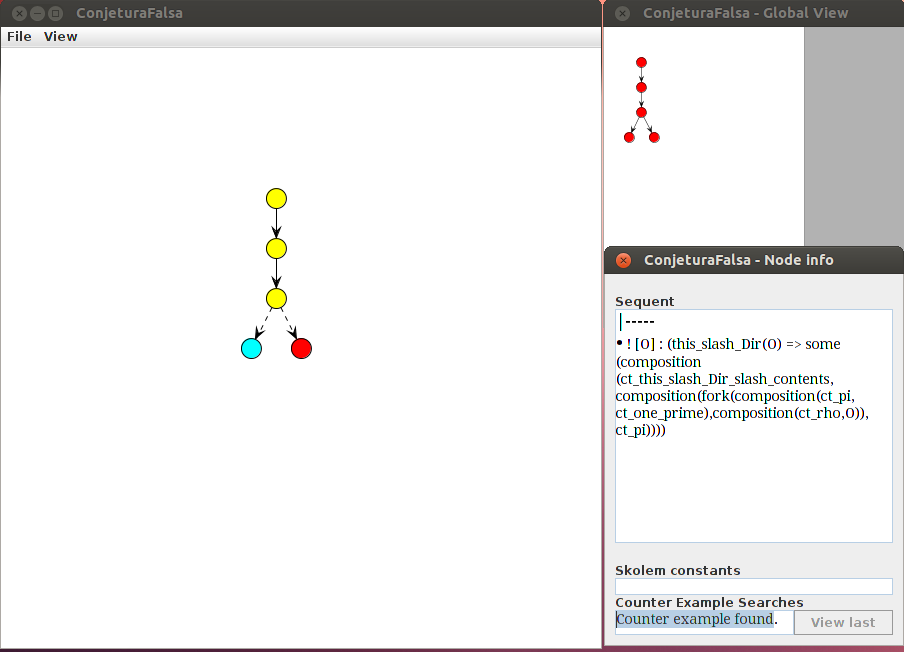
\includegraphics[width=350px]{img/conjetura_falsa_4.png}
	\centering
	\caption{El nodo rojo indica que se encontr'o un contraejemplo}
\end{figure}

Al encontrar un contraejemplo en una ramificaci'on alternativa, se puede afirmar que existe un contraejemplo para el nodo ra'iz de la ramificaci'on. Luego el contraejemplo es para el secuente en el lenguaje \textit{TPTP-FOF}, pero como es un lenguaje menos expresivo que \textit{PDOCFA} entonces tambi'en existe un contraejemplo para el secuente en \textit{PDOCFA}. Adem'as como la traducci'on entre \textit{Alloy} y \textit{PDOCFA} es sin p'erdida de precisi'on, existe un contraejemplo para el secuente original en \textit{Alloy}. Con lo cu'al se concluye que la conjetura es falsa.


\section{Analisis de lemas XXX}
\todomm{XXX: Mencionar que estos lemas forman parte de las demostraciones realizadas con Dynamite.}
\label{analisis_lemas}
Como parte del an'alisis y evaluaci'on de los demostradores de teoremas integrados (\textit{EProver} y \textit{SPASS}) evaluamos un conjunto de lemas correspondientes a XXX \ref{anexo_lemas_fof}.

Los lemas se definieron como f'ormulas \textit{PDOCFA}, se aplic'o una traducci'on-$\rho$ a \textit{TPTP-FOF} y se trat'o de demostrar cada lema por separado. C'omo la traducci'on entre \textit{PDOCFA} y \textit{TPTP-FOF} no es exacta, fue necesario especificar un par'ametro numerico $n$ que indica la cantidad de desarrollos que se hacen de la clausura reflexotransitiva. Para 'estos ejemplos probamos con el par'ametro $n$=$5$, $10$, $20$ y $50$. En todos los casos obtuvimos los mismos resultados:

\vspace{1em}
\begin{verbnobox}[\tiny]
M1:
	FORALL (A: Carrier| Leq(A,univ),
		   R: Carrier|  ( Leq(R,CartesianProduct(univ,univ,1,1)) AND Leq(R,CartesianProduct(A,A,1,1)) ) ,
		   S: Carrier|  ( Leq(S,CartesianProduct(univ,univ,1,1)) AND Leq(S,CartesianProduct(A,A,1,1)) ) ):
	  (FORALL (a0: Carrier|  (  ( Leq(a0,univ) AND Leq(a0,A) )  AND One(a0) ), 
			   af: Carrier|  (  ( Leq(af,univ) AND Leq(af,A) )  AND One(af) ) ) : 
		  ( ( ( ( ( Leq(af,Navigation(a0,TC(sum(R,S)),1,2)) AND
			None(product(Navigation(A,S,1,2),Navigation(R,A,2,1))) ) AND
		    None(product(Navigation(S,A,2,1),Navigation(R,A,2,1))) )
		  IMPLIES 
			Leq(af,Navigation(a0,TC(R),1,2)) ) OR 
			Leq(af,Navigation(a0,TC(S),1,2)) ) OR
			(EXISTS (ai: Carrier|  (  ( Leq(ai,univ) AND Leq(ai,A) )  AND One(ai) ) ) : 
				( Leq(ai,Navigation(a0,TC(R),1,2)) AND Leq(af,Navigation(ai,TC(S),1,2)) ) ) ) ))
\end{verbnobox}

\begin{verbnobox}[\tiny]
M10:
	FORALL (A: Carrier| Leq(A,univ), 
		   B: Carrier| Leq(B,univ), 
		   C: Carrier| Leq(C,univ), 
		   W: Carrier| Leq(W,CartesianProduct(A,CartesianProduct(B,C,1,1),1,2)), 
		   a: Carrier| ( Leq(a,A) AND One(a) ) ) : 
	  Leq(Navigation(a,W,1,3),CartesianProduct(B,C,1,1))

\end{verbnobox}

\begin{verbnobox}[\tiny]
M11b:	
	FORALL (A: Carrier| Leq(A,univ), 
		   B: Carrier| Leq(B,univ), 
		   R: Carrier| Leq(R,CartesianProduct(A,B,1,1))) : Leq(Navigation(a,R,1,2),B))
\end{verbnobox}

\begin{verbnobox}[\tiny]
M12b:
 FORALL (A,B,C: Carrier):( Leq(A,C) AND Leq(B,C) ) => Leq(sum(A, B),C)
\end{verbnobox}

\begin{verbnobox}[\tiny]
M13:	
	FORALL (A: Carrier| Leq(A,univ), 
		   B: Carrier| Leq(B,univ), 
		   R: Carrier| Leq(R,CartesianProduct(A,B,1,1))) : 
	  Leq(RTC(R),CartesianProduct(A,B,1,1))
\end{verbnobox}

\begin{verbnobox}[\tiny]
M15:
	THEOREM FORALL (A: Carrier| Leq(A,univ), 
				   B: Carrier| Leq(B,univ), 
				   R: Carrier| Leq(R,CartesianProduct(A,B,1,1)), 
				   S: Carrier| Leq(S,CartesianProduct(A,B,1,1)), 
				   C: Carrier| ( Leq(C,A) AND One(C) ) ) :  
			( Leq(R,S) IMPLIES Leq(Navigation(C,R,1,2),Navigation(C,S,1,2)) )
\end{verbnobox}

\begin{verbnobox}[\tiny]
M16:
	FORALL (A,B: Carrier) : Leq(A,sum(A, B))
\end{verbnobox}

\begin{verbnobox}[\tiny]
M17:
	THEOREM FORALL (A: Carrier| Leq(A,univ), 
				    B: Carrier| Leq(B,univ), 
				    R: Carrier| Leq(R,CartesianProduct(A,B,1,1)), 
				    S: Carrier| Leq(S,CartesianProduct(A,B,1,1))) :  
		 	Leq(R,S) IMPLIES Leq(RTC(R),RTC(S))  
\end{verbnobox}

\begin{verbnobox}[\tiny]
M18:
	FORALL (A,x: Carrier) : (None(A) & Some(x)) => NotLeq(x,A)
\end{verbnobox}

\begin{verbnobox}[\tiny]
M19:
	FORALL (A: Carrier| Leq(A,univ), 
		    B: Carrier| Leq(B,univ), 
		    R: Carrier| Leq(R,CartesianProduct(A,B,1,1))) : Leq(Navigation(R,B,2,1),A)
\end{verbnobox}

\begin{verbnobox}[\tiny]
M1h0:
	FORALL (A: Carrier| Leq(A,univ), 
			R: Carrier| ( Leq(R,CartesianProduct(univ,univ,1,1)) AND Leq(R,CartesianProduct(A,A,1,1)) ), 
			S: Carrier| ( Leq(S,CartesianProduct(univ,univ,1,1)) AND Leq(S,CartesianProduct(A,A,1,1)) ) ) : 
	  (  ( None(product(Navigation(A,S,1,2),Navigation(R,A,2,1))) 
			AND None(product(Navigation(S,A,2,1),Navigation(R,A,2,1))) )  
      IMPLIES  
      	( TC(sum(R,S)) = sum(sum(TC(R),TC(S)),Navigation(TC(R),TC(S),2,2)) )  ))
\end{verbnobox}

\begin{verbnobox}[\tiny]
M1M1:
	FORALL (A: Carrier| Leq(A,univ), 
			R: Carrier | ( Leq(R,CartesianProduct(univ,univ,1,1)) AND Leq(R,CartesianProduct(A,A,1,1)) ),
			S: Carrier | ( Leq(S,CartesianProduct(univ,univ,1,1)) AND Leq(S,CartesianProduct(A,A,1,1)) ) )
	:(FORALL (a0: Carrier | ( ( Leq(a0,univ) AND Leq(a0,A) ) AND One(a0) ),
			  af: Carrier | ( ( Leq(af,univ) AND Leq(af,A) ) AND One(af) ) )
		: ( ( ( ( Leq(af,Navigation(a0,TC(sum(R,S)),1,2)) AND
				  None(product(Navigation(A,S,1,2),Navigation(R,A,2,1))) ) AND
				  None(product(Navigation(S,A,2,1),Navigation(R,A,2,1))) ) AND
				  Leq(a0,Navigation(S,A,2,1)) )
						IMPLIES Leq(af,Navigation(a0,TC(S),1,2)) ) ))
\end{verbnobox}

\begin{verbnobox}[\tiny]
M1M1b:
		
	FORALL (A: Carrier| Leq(A,univ), 
			R: Carrier | ( Leq(R,CartesianProduct(univ,univ,1,1)) AND Leq(R,CartesianProduct(A,A,1,1)) ),
			S: Carrier | ( Leq(S,CartesianProduct(univ,univ,1,1)) AND Leq(S,CartesianProduct(A,A,1,1)) ) )
	:(FORALL (a0: Carrier | ( ( Leq(a0,univ) AND Leq(a0,A) ) AND One(a0) ),
			  af: Carrier | ( ( Leq(af,univ) AND Leq(af,A) ) AND One(af) ) )
		: ( ( ( ( Leq(af,Navigation(a0,RTC(sum(R,S)),1,2)) AND
				  None(product(Navigation(A,S,1,2),Navigation(R,A,2,1))) ) AND
				  None(product(Navigation(S,A,2,1),Navigation(R,A,2,1))) ) AND
				  Leq(a0,Navigation(S,A,2,1)) )
						IMPLIES Leq(af,Navigation(a0,RTC(S),1,2)) ) ))
\end{verbnobox}

\begin{verbnobox}[\tiny]
M1M4:
	FORALL (A: Carrier| Leq(A,univ), 
		   R: Carrier| ( Leq(R,CartesianProduct(univ,univ,1,1)) AND Leq(R,CartesianProduct(A,A,1,1)) ) , 
		   S: Carrier| ( Leq(S,CartesianProduct(univ,univ,1,1)) AND Leq(S,CartesianProduct(A,A,1,1)) ) ) : 
	  (FORALL (a0: Carrier|  (  ( Leq(a0,univ) AND Leq(a0,A) )  AND One(a0) ) , 
			   af: Carrier|  (  ( Leq(af,univ) AND Leq(af,A) )  AND One(af) ) ) : 
		  (  
			 ( Leq(af,Navigation(a0,TC(sum(R,S)),1,2)) AND 
		  	 (FORALL (ai: Carrier|  (  ( Leq(ai,univ) AND Leq(ai,A) ) AND One(ai) ) ) :  
					(  ( Leq(ai,Navigation(a0,RTC(sum(R,S)),1,2)) AND 
					Leq(af,Navigation(ai,RTC(sum(R,S)),1,2)) ) 
					IMPLIES NOT ( Leq(ai,Navigation(S,A,2,1)) )  ) ) )
			IMPLIES Leq(af,Navigation(a0,TC(R),1,2)) ) )
\end{verbnobox}

\begin{verbnobox}[\tiny]
M1M5:
	FORALL (A: Carrier| Leq(A,univ), 
		   R: Carrier| ( Leq(R,CartesianProduct(univ,univ,1,1)) AND Leq(R,CartesianProduct(A,A,1,1)) ) , 
		   S: Carrier| ( Leq(S,CartesianProduct(univ,univ,1,1)) AND Leq(S,CartesianProduct(A,A,1,1)) ) ) : 
	  (FORALL (a0: Carrier|  (  ( Leq(a0,univ) AND Leq(a0,A) )  AND One(a0) ) , 
			   af: Carrier|  (  ( Leq(af,univ) AND Leq(af,A) )  AND One(af) ) ) : 
		  (
			 ( Leq(af,Navigation(a0,RTC(sum(R,S)),1,2))) AND 
		  	 (EXISTS (ai: Carrier|  (  ( Leq(ai,univ) AND Leq(ai,A) ) AND One(ai) ) ) :  
					(  ( Leq(ai,Navigation(a0,RTC(sum(R,S)),1,2)) AND 
						 Leq(af,Navigation(ai,RTC(sum(R,S)),1,2)) ) AND
						 Leq(ai,Navigation(S,A,2,1)) ) ) 
		  )  
		 	IMPLIES (EXISTS (aj: Carrier|  (  ( Leq(aj,univ) AND Leq(aj,A) )  AND One(aj) ) ) : 
				(  ( Leq(aj,Navigation(a0,RTC(R),1,2)) AND 
					 Leq(af,Navigation(aj,RTC(sum(R,S)),1,2)) ) AND 
					 Leq(aj,Navigation(S,A,2,1)) ) ) ) )) 
\end{verbnobox}

\begin{verbnobox}[\tiny]
M1M6:
	FORALL (A: Carrier| Leq(A,univ), 
				    U: Carrier| ( Leq(U,CartesianProduct(univ,univ,1,1)) AND Leq(U,CartesianProduct(A,A,1,1)) ) ): 
	   (FORALL (i: Carrier|  (  ( Leq(i,univ) AND Leq(i,A) )  AND One(i) ) , 
				j: Carrier|  (  ( Leq(j,univ) AND Leq(j,A) )  AND One(j) ) ) :
		(Leq(i,Navigation(j,TC(U),1,2))
		IMPLIES 
			(EXISTS (k: Carrier|  (  ( Leq(k,univ) AND Leq(k,A) )  AND One(k) ) ) : 
				(Leq(k,Navigation(j,RTC(U),1,2)) AND Leq(i,Navigation(k,U,1,2)) ) ) ) )
\end{verbnobox}

\begin{verbnobox}[\tiny]
M1M7:
	FORALL (A: Carrier| Leq(A,univ), 
		   U: Carrier| (Leq(U,CartesianProduct(univ,univ,1,1)) AND Leq(U,CartesianProduct(A,A,1,1)) ),
		   T: Carrier| (Leq(T,CartesianProduct(univ,univ,1,1)) AND Leq(T,CartesianProduct(A,A,1,1)) ) ) : 
	  (FORALL (i: Carrier|  (  ( Leq(i,univ) AND Leq(i,A) )  AND One(i) ) , 
			   j: Carrier|  (  ( Leq(j,univ) AND Leq(j,A) )  AND One(j) ) ) : 
		  ( Leq(i,Navigation(j,RTC(U),1,2)) IMPLIES Leq(i,Navigation(j,RTC(sum(U,T)),1,2)) ) ))
\end{verbnobox}

\begin{verbnobox}[\tiny]
M2:	
	FORALL (A: Carrier| Leq(A,univ), 
		   B: Carrier| Leq(B,univ), 
		   R: Carrier| ( Leq(R,CartesianProduct(univ,univ,1,1)) AND Leq(R,CartesianProduct(univ,B)) ) , 
		   S: Carrier| ( Leq(S,CartesianProduct(univ,univ,1,1)) AND Leq(S,CartesianProduct(univ,A)) ) ) : 
	  (FORALL (a: (atom), 
			   c: Carrier| ( ( Leq(c,univ) AND Leq(c,B) )  AND One(c) ) , 
			   d: Carrier| ( ( Leq(d,univ) AND Leq(d,A) )  AND One(d) ) ) :  
			(  ( Leq(c,Navigation(a,R,1,2)) AND Leq(d,Navigation(A,S,1,2)) )  IMPLIES 
					Some(product(Navigation(R,B,2,1),Navigation(S,A,2,1))) ) ))
\end{verbnobox}

\begin{verbnobox}[\tiny]
M20:
 	atom(X) = One(X)
	FORALL (A: Carrier| Leq(A,univ), B: Carrier| Leq(B,univ), x: (atom)):
		 ( Leq(x,sum(A,B)) => ( Leq(x,A) OR Leq(x,B) ))
\end{verbnobox}

\begin{verbnobox}[\tiny]
M21:
	FORALL (A: Carrier| Leq(A,univ), 
		   B: Carrier| Leq(B,univ), 
		   C: Carrier| Leq(C,univ), 
		   D: Carrier| Leq(D,univ)) :
  ( ( Leq(A,B) AND Leq(C,D) )  IMPLIES Leq(CartesianProduct(A,C,1,1),CartesianProduct(B,D,1,1)) ) )
\end{verbnobox}

\begin{verbnobox}[\tiny]
M22:
	FORALL (A: Carrier| Leq(A,univ), 
		   B: Carrier| Leq(B,univ), 
		   R: Carrier| Leq(R,CartesianProduct(A,B,1,1)), 
		   S: Carrier| Leq(S,CartesianProduct(A,B,1,1))) : 
	  ( sum(Navigation(R,B,2,1),Navigation(S,B,2,1)) = Navigation(sum(R,S),B,2,1) )
\end{verbnobox}

\begin{verbnobox}[\tiny]
M23:
	FORALL (A: Carrier| Leq(A,univ), B: Carrier| Leq(B,univ)) :
		( None(sum(A,B)) IFF  ( None(A) AND None(B) )  ) )
\end{verbnobox}

\begin{verbnobox}[\tiny]
M23b:
	FORALL (A: Carrier| Leq(A,univ), 
		   B: Carrier| Leq(B,univ), 
		   C: Carrier| Leq(C,univ), 
		   R: Carrier| Leq(R,CartesianProduct(A,B,1,1)), 
		   a: Carrier|  ( Leq(a,A) AND One(a) ) ) :
	 ( ( Leq(a,C) AND None(product(Navigation(R,B,2,1),C)) ) IMPLIES None(Navigation(a,R,1,2)) )
\end{verbnobox}

\begin{verbnobox}[\tiny]
M24:
	FORALL (A: Carrier| Leq(A,univ), 
		   B: Carrier| Leq(B,univ), 
		   R: Carrier| ( Leq(R,CartesianProduct(univ,univ,1,1)) AND Leq(R,CartesianProduct(A,B,1,1)) ) , 
		   S: Carrier|  ( Leq(S,CartesianProduct(univ,univ,1,1)) AND Leq(S,CartesianProduct(A,B,1,1)) ) ) :
		( sum(Navigation(a,R,1,2),Navigation(A,S,1,2)) = Navigation(A,sum(R,S),1,2) ) )
\end{verbnobox}

\begin{verbnobox}[\tiny]
M25:
	FORALL (A: Carrier, B: Carrier, C: Carrier) :  
			( (Leq(A,C)) AND (Leq(B,C)) )  IMPLIES (Leq(product(A, B),C)) )
\end{verbnobox}

\begin{verbnobox}[\tiny]
M30:
	FORALL (A: Carrier| Leq(A,univ), 
		   B: Carrier| Leq(B,univ), 
		   R: Carrier| (Leq(R,CartesianProduct(univ,univ,1,1)) AND Leq(R,CartesianProduct(A,B,1,1)) ), 
		   a: Carrier| (( Leq(a,univ) AND Leq(a,A) )  AND One(a) ) ) : 
	  Leq(a,Navigation(a,RTC(R),1,2)))
\end{verbnobox}

\begin{verbnobox}[\tiny]
M31:
	FORALL (A: Carrier| Leq(A,univ), 
		   B: Carrier| Leq(B,univ), 
		   R: Carrier|  ( Leq(R,CartesianProduct(univ,univ,1,1)) AND Leq(R,CartesianProduct(A,B,1,1)) ),
		   x: Carrier|  (  ( Leq(x,univ) AND Leq(x,A) )  AND One(x) ),
		   y: Carrier|  (  ( Leq(y,univ) AND Leq(y,A) )  AND One(y) ) ) : 
	  ( Leq(y,Navigation(x,TC(R),1,2)) IMPLIES Leq(y,Navigation(x,RTC(R),1,2)) )
\end{verbnobox}

\begin{verbnobox}[\tiny]
M32:
	FORALL (A: Carrier| Leq(A,univ),
		   B: Carrier| Leq(B,univ), 
		   R: Carrier|  ( Leq(R,CartesianProduct(univ,univ,1,1)) AND Leq(R,CartesianProduct(A,B,1,1)) ),
		   S: Carrier|  ( Leq(S,CartesianProduct(univ,univ,1,1)) AND Leq(S,CartesianProduct(A,B,1,1)) ),
		   x: Carrier|  (  ( Leq(x,univ) AND Leq(x,A) )  AND One(x) ) ) : 
	  ( Leq(x,Navigation(R,B,2,1)) IMPLIES Leq(x,Navigation(sum(R,S),B,2,1)) ) )
\end{verbnobox}

\begin{verbnobox}[\tiny]	
M4:
	FORALL (A: Carrier| Leq(A,univ), 
		   U: Carrier| ( Leq(U,CartesianProduct(univ,univ,1,1)) AND Leq(U,CartesianProduct(A,A,1,1)) ) ) : 
	  (FORALL (i: Carrier|  (  ( Leq(i,univ) AND Leq(i,A) )  AND One(i) ) , 
			   j: Carrier|  (  ( Leq(j,univ) AND Leq(j,A) )  AND One(j) ) ) :  
			( Leq(i,Navigation(j,TC(U),1,2)) IMPLIES 
				(EXISTS (k: Carrier|  (  ( Leq(k,univ) AND Leq(k,A) )  AND One(k) ) ) :  
					( Leq(k,Navigation(j,U,1,2)) AND Leq(i,Navigation(k,RTC(U),1,2)) ) ) ) )
\end{verbnobox}

\begin{verbnobox}[\tiny]
M5FORALL:
	(A: Carrier| Leq(A,univ), 
		   R: Carrier|  ( Leq(R,CartesianProduct(univ,univ,1,1)) AND Leq(R,CartesianProduct(A,A,1,1)) ) ) : 
  ( None(product(Navigation(a,R,1,2),Navigation(R,A,2,1))) IMPLIES None(product(TC(R),iden)) ) )
\end{verbnobox}

\begin{verbnobox}[\tiny]
M5M1:
	FORALL (A: Carrier| Leq(A,univ), 
		   R: Carrier| ( Leq(R,CartesianProduct(univ,univ,1,1)) AND Leq(R,CartesianProduct(A,A,1,1)) ),
		   S: Carrier| ( Leq(S,CartesianProduct(univ,univ,1,1)) AND Leq(S,CartesianProduct(A,A,1,1)) ) ) : 
   ( None(product(Navigation(A,S,1,2),Navigation(R,A,2,1))) 
   IMPLIES None(product(Navigation(TC(R),TC(S),2,2),iden)) ) )
\end{verbnobox}

\begin{verbnobox}[\tiny]
M6M1r2:
	FORALL (A: Carrier| Leq(A,univ),
		   R: Carrier| ( Leq(R,CartesianProduct(univ,univ,1,1)) AND Leq(R,CartesianProduct(A,A,1,1)) ),
		   S: Carrier| ( Leq(S,CartesianProduct(univ,univ,1,1)) AND Leq(S,CartesianProduct(A,A,1,1)) ) ): 
		(  ( None(R) AND None(S) )  IMPLIES None(sum(R,S)) ) )
\end{verbnobox}

\begin{verbnobox}[\tiny]
M6M1r2b:
	FORALL (R: Carrier, S: Carrier ) :  (  ( None(R) AND None(S) )  IMPLIES None(sum(R,S)) ) )
\end{verbnobox}

\begin{verbnobox}[\tiny]
M6M1r2c:
	FORALL (R: Carrier, S: Carrier ) :  (  None(sum(R,S)) IMPLIES ( None(R) AND None(S) ) ) )
\end{verbnobox}

\begin{verbnobox}[\tiny]
M7:
	FORALL (A: Carrier| Leq(A,univ),
		   R: Carrier|  ( Leq(R,CartesianProduct(univ,univ,1,1)) AND Leq(R,CartesianProduct(A,A,1,1)) ) ,
		   a: Carrier|  (  ( Leq(a,univ) AND Leq(a,A) )  AND One(a) ),
		   b: Carrier|  (  ( Leq(b,univ) AND Leq(b,A) )  AND One(b) ),
		   c: Carrier|  (  ( Leq(c,univ) AND Leq(c,A) )  AND One(c) ) ):
		((((((FORALL (d: Carrier|  (  ( Leq(d,univ) AND Leq(d,A) )  AND One(d) ) ): Lone(Navigation(d,R,1,2)))
		AND 
			Leq(b,Navigation(a,TC(R),1,2)) ) AND 
			Leq(c,Navigation(a,TC(R),1,2)) )  AND NotEquals(b,c) ) 
	    IMPLIES Leq(b,Navigation(c,TC(R),1,2)) )  OR Leq(c,Navigation(b,TC(R),1,2)) ) )
\end{verbnobox}

\begin{verbnobox}[\tiny]
M8:
	FORALL (A: Carrier| Leq(A,univ), 
		   R: Carrier|  ( Leq(R,CartesianProduct(univ,univ,1,1)) AND Leq(R,CartesianProduct(A,A,1,1)) ) ) : 
    (FORALL (a: Carrier|  (  ( Leq(a,univ) AND Leq(a,A) )  AND One(a) ) , 
    		    b: Carrier|  (  ( Leq(b,univ) AND Leq(b,A) )  AND One(b) ) ) : 
    	    (  ( Leq(b,Navigation(a,RTC(R),1,2)) AND NotEquals(a,b) )
    			IMPLIES Leq(b,Navigation(a,TC(R),1,2)) ) )
\end{verbnobox}

\begin{verbnobox}[\tiny]
M9:
	Forall(A,B,C : Carrier) : (Leq(A,B) AND Leq(B,C)) => Leq(A,C)
\end{verbnobox}

\begin{verbnobox}[\tiny]
Mb2:
	FORALL (A: Carrier| Leq(A,univ), 
		   B: Carrier| Leq(B,univ), 
		   R: Carrier| (Leq(R,CartesianProduct(univ,univ,1,1)) AND Leq(R,CartesianProduct(A,B,1,1)) ),
		   S: Carrier| (Leq(S,CartesianProduct(univ,univ,1,1)) AND Leq(S,CartesianProduct(A,B,1,1)) ) ) :
	   (( ( (FORALL (a: Carrier|  (  ( Leq(a,univ) AND Leq(a,A) )  AND One(a) ) ) : 
			Lone(Navigation(a,R,1,2))) 
		    AND 
			(FORALL (a: Carrier|  (  ( Leq(a,univ) AND Leq(a,A) )  AND One(a) ) ) : 
				Lone(Navigation(A,S,1,2))) ) AND None(product(Navigation(R,B,2,1),Navigation(S,B,2,1))) 
	    )
		IMPLIES (FORALL (a: Carrier|  (  ( Leq(a,univ) AND Leq(a,A) )  AND One(a) ) ) : 
		    Lone(Navigation(A,sum(R,S),1,2))) ) )
\end{verbnobox}
\vspace{1em}

De 'esto lemas los que se pudieron demostrar automaticamente tanto por \textit{E-Prover} como por \textit{SPASS} son: M9, M6M1r2b, M6M1r2c, M6M1r2, M25, M23, M16, M12b.

Tanto \textit{EProver} como \textit{SPASS} tuvieron el mismo comportamiento y lograron demostrar los mismos lemas.

Analizando cada lema se puede ver que los lemas que fueron demostrados no contienen la operaci'on \textbf{composition}. A su vez los lemas que no tuvieron un resultado positivo, todos conten'ian dicha operaci'on. 

Creemos que el problema reside ah'i, ya que los demostradores tanto \textit{EProver} como  \textit{SPASS} son generales para l'ogica de primer 'orden y es necesario usar t'ecnicas de demostraci'on especificas de 'algebras relacionales al trabajar con las composiciones. En caso contrario, el demostrador puede entrar en un ciclo infinito buscando como realizar la composici'on.


%á